\documentclass[tikz,border=8pt]{standalone}
\usepackage{amsmath}
\usetikzlibrary{arrows.meta,decorations.pathreplacing}
\begin{document}

% Asset ID: AS2DataPresentationTikZ-002
% Source: Outlier rule evidence.
% Related lesson section: Core Theory, Outliers.
% Purpose: Show outlier boundaries using Q_1 - 1.5IQR and Q_3 + 1.5IQR.
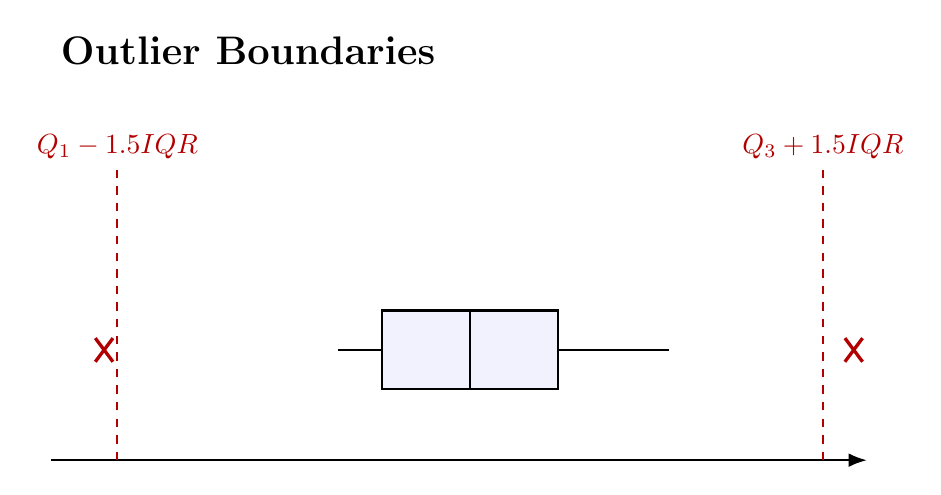
\begin{tikzpicture}[x=0.28cm,y=1cm,>=Latex,font=\sffamily]
\node[anchor=west,font=\bfseries\Large] at (-5,5.2) {Outlier Boundaries};
\draw[->,thick] (-5,0)--(32,0);
\draw[thick] (8,1.4)--(10,1.4); \draw[thick] (18,1.4)--(23,1.4); \draw[thick,fill=blue!5] (10,0.9) rectangle (18,1.9); \draw[thick] (14,0.9)--(14,1.9);
\draw[dashed,red!70!black,thick] (-2,0)--(-2,3.7); \draw[dashed,red!70!black,thick] (30,0)--(30,3.7);
\node[above,red!70!black] at (-2,3.7){$Q_1-1.5IQR$}; \node[above,red!70!black] at (30,3.7){$Q_3+1.5IQR$};
\draw[red!70!black,very thick] (-3,1.25)--(-2.2,1.55); \draw[red!70!black,very thick] (-3,1.55)--(-2.2,1.25);
\draw[red!70!black,very thick] (31,1.25)--(31.8,1.55); \draw[red!70!black,very thick] (31,1.55)--(31.8,1.25);
\end{tikzpicture}

\end{document}
